% called by main.tex
%
\chapter{Alineación Mediante Optimización de Preferencias Directa}
\label{ch::chapter7}

El capítulo anterior mostró que las variantes con cabezal explícito de nivel son metodológicamente
interesantes, pero no constituyen todavía la base más estable para una fase posterior de alineación.
Por ese motivo, la etapa de DPO se aplica sobre el mejor modelo operativo disponible:
\texttt{serialized\_sft}. La pregunta cambia ligeramente respecto a los capítulos anteriores. Ya no se
trata de comprobar si el modelo puede aprender la superficie estructurada básica, sino de estudiar si
un modelo que ya genera \texttt{blocks\_tsv\_v1} de forma competente puede refinarse mediante
preferencias automáticas sin perder la estabilidad estructural que lo hace útil.

DPO (\textit{Direct Preference Optimization}) permite ajustar una política a partir de pares de
respuestas preferidas y rechazadas sin entrenar un modelo de recompensa separado ni ejecutar una fase
de refuerzo \textit{online} \citep{rafailov2023dpo}. En este trabajo, esas preferencias no proceden de
juicios humanos, sino de señales automáticas derivadas del parser, de la adecuación al prompt y de los
checks de dominio Kubernetes. Precisamente por eso, antes de hablar del etiquetado de pares o del
entrenamiento DPO, es necesario justificar cómo se generó el conjunto de candidatos sobre el que se
construyeron esas preferencias.

%----------------------------------------------------------------------
\section{Generación de candidatos para DPO}
\label{sec:ch7_candidate_generation}
%----------------------------------------------------------------------

La construcción de un dataset de preferencias no empieza con el etiquetado, sino con una decisión
más básica: cuántas salidas generar para cada prompt y con qué nivel de diversidad. Si el modelo
produce candidatos demasiado parecidos, la comparación entre salidas apenas aporta señal. Si, por el
contrario, la decodificación es demasiado agresiva, los pares resultantes pueden quedar dominados por
errores triviales de formato o de parseabilidad. El objetivo de esta fase fue encontrar un punto
intermedio: generar suficientes variantes por prompt para que aparezcan contrastes útiles, pero sin
salir de la distribución aprendida por \texttt{serialized\_sft}.

Para ello se probaron varias estrategias de muestreo sobre el split de entrenamiento. La primera
familia generaba cuatro candidatos por prompt con temperaturas moderadas. La segunda ampliaba a seis
candidatos, pero mantenía un rango bajo-medio de temperatura. La tercera, que acabó siendo la base
del conjunto final, también generaba seis candidatos, pero cubría un rango más amplio:
\(0{,}45\), \(0{,}65\), \(0{,}85\), \(1{,}0\), \(1{,}1\) y \(1{,}2\), con \texttt{top\_p=0.95}.
La Figura~\ref{fig:ch7_candidate_strategy_comparison} resume la comparación entre estas estrategias.

\begin{figure}[htbp]
\centering
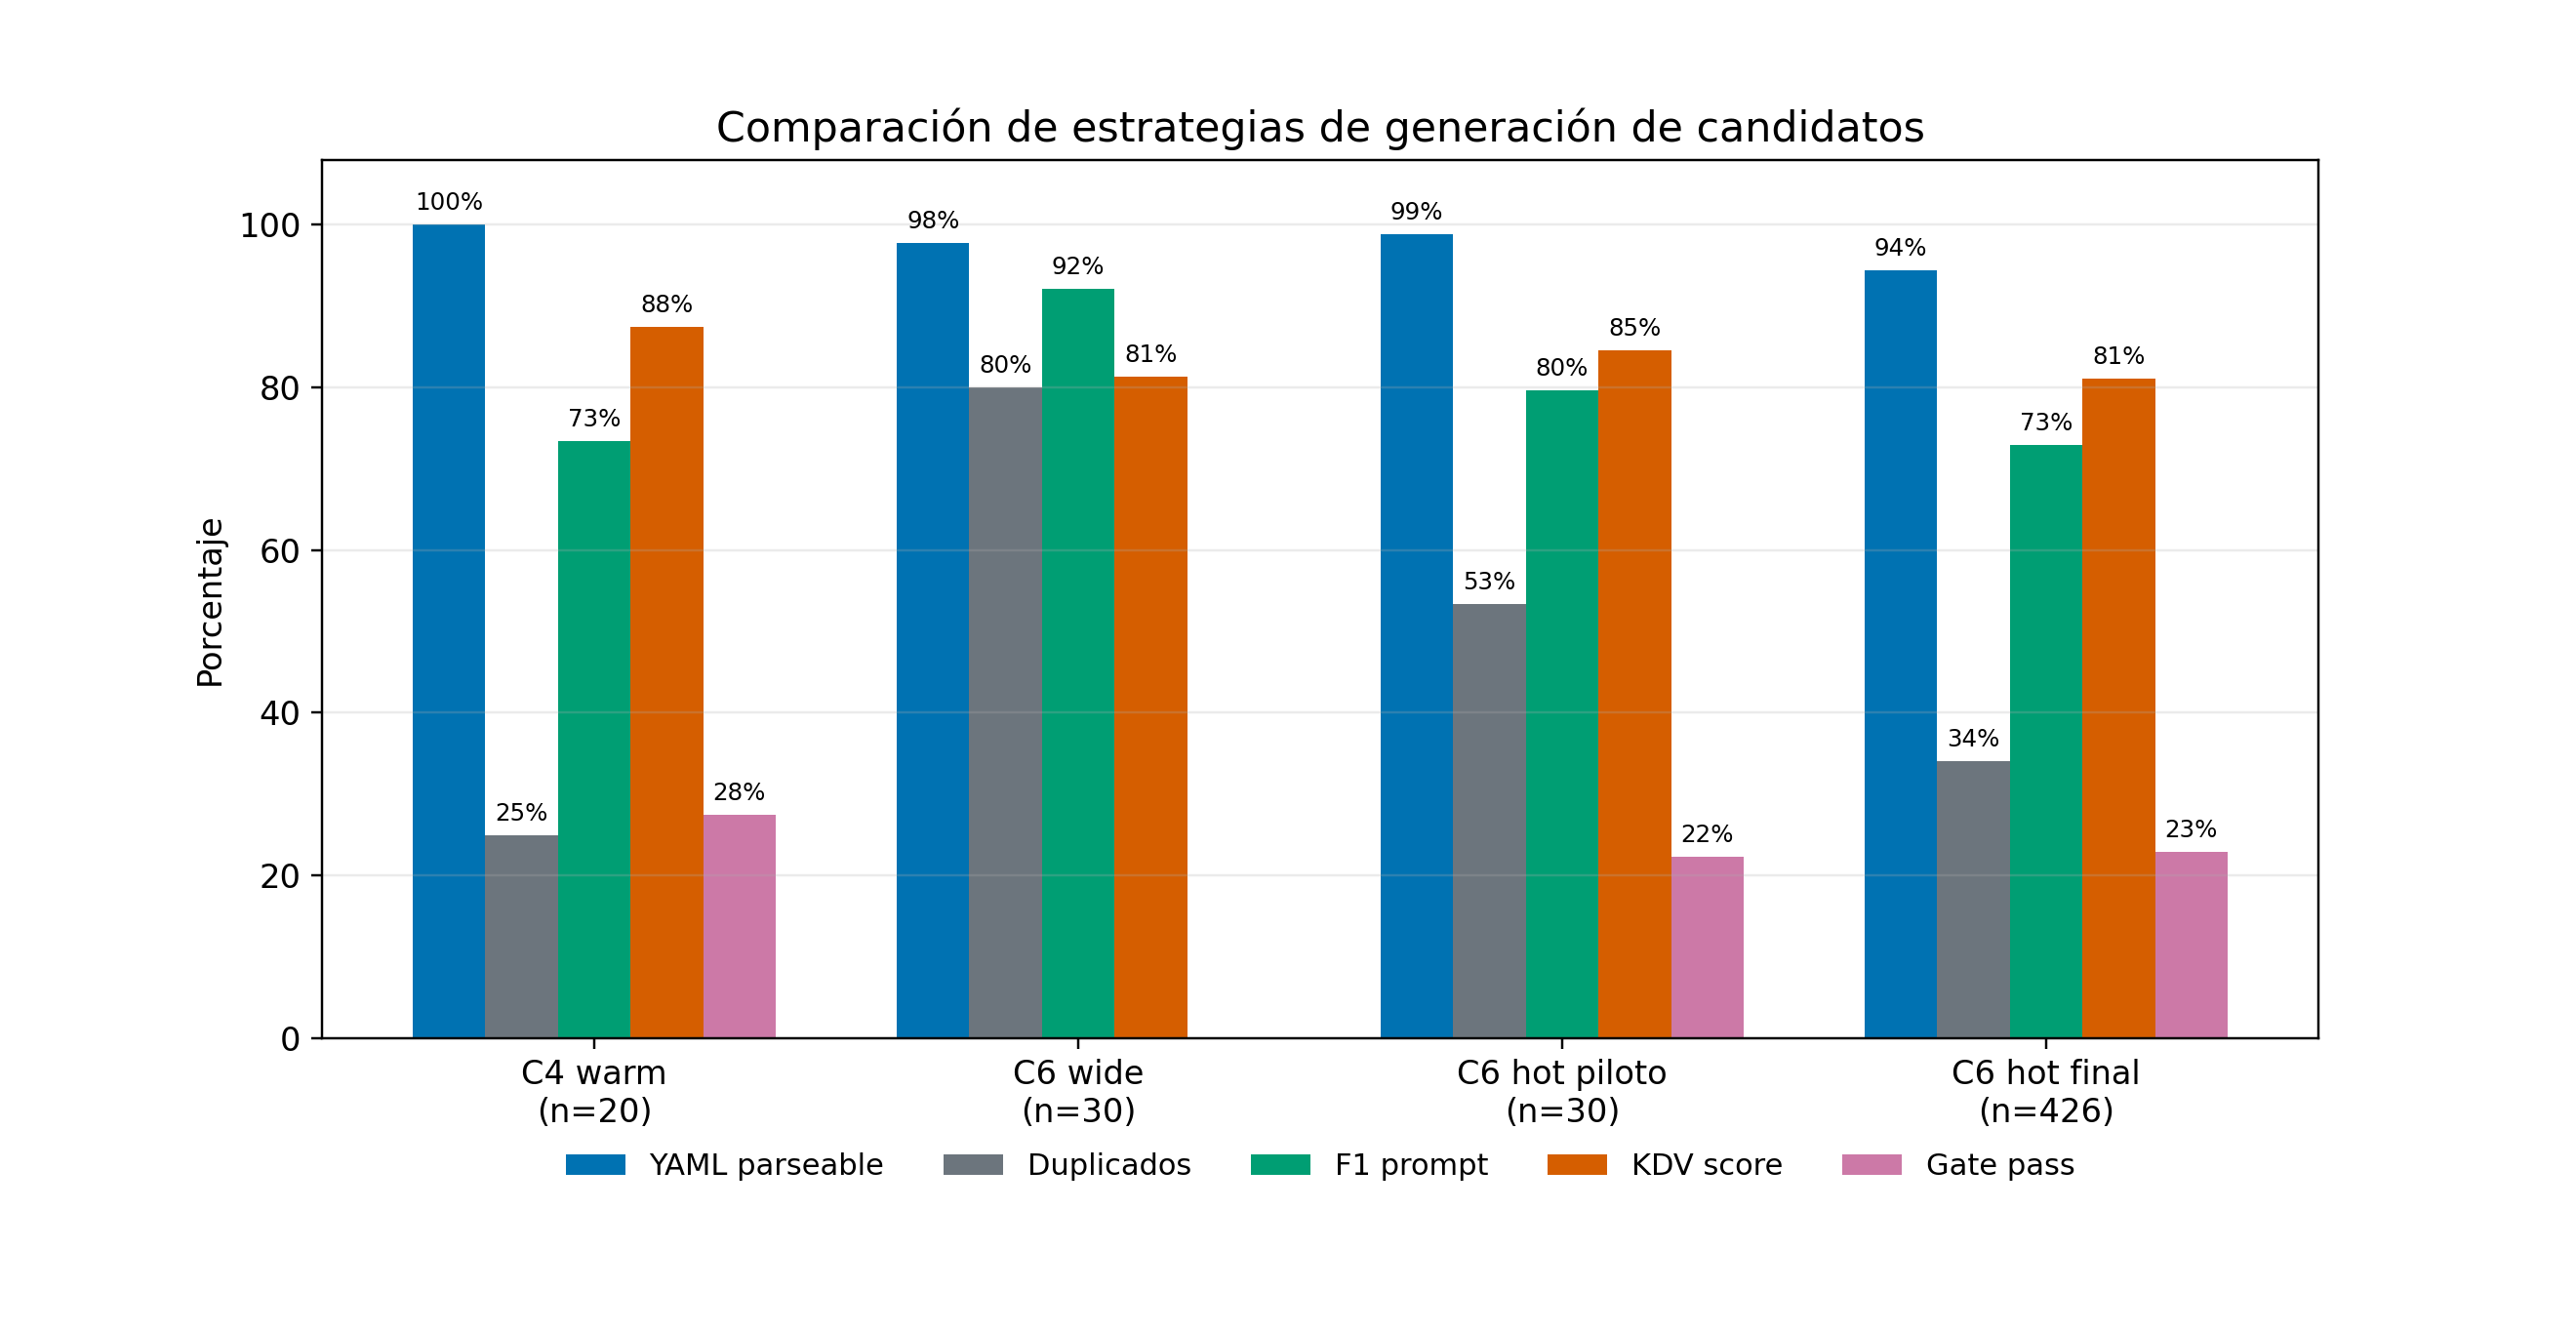
\includegraphics[width=\textwidth]{figures/chapter7/fig7_1_candidate_strategy_comparison.png}
\caption{Comparación de estrategias de generación de candidatos para DPO. Los pilotos se ejecutaron
         sobre subconjuntos distintos, por lo que deben leerse como una exploración metodológica y no
         como una comparación controlada exacta. La fila \texttt{C6 hot final} agrega las 426 unidades
         de prompt usadas en la generación principal.}
\label{fig:ch7_candidate_strategy_comparison}
\end{figure}

La lectura principal no es que una estrategia maximice todas las métricas a la vez, sino que cada una
ofrece un equilibrio distinto. El piloto \texttt{C6 wide} conserva una adecuación al prompt muy alta
(92~\%), pero genera una tasa de duplicados también elevada. El rango \texttt{C6 hot}, en cambio, reduce la fidelidad
media al prompt, pero introduce más variabilidad y recupera candidatos que sí pasan el \textit{gate}
Kubernetes. Esta diferencia es importante porque DPO no necesita únicamente buenas salidas; necesita
pares comparables donde una salida sea preferible a otra por razones reconocibles.

El análisis por temperatura confirma esa tensión. Como muestra la
Figura~\ref{fig:ch7_metrics_by_temperature}, las temperaturas bajas mantienen mejor parseabilidad,
mejor F1 de prompt y mayor score preferencial medio. A \(0{,}45\) y \(0{,}65\), la tasa de YAML
parseable se mantiene cerca del 99~\%, mientras que a \(1{,}2\) cae al 87~\% y aumenta la
proporción de candidatos inválidos. Sin embargo, las temperaturas altas no se descartan por completo:
su utilidad no está en producir el mejor candidato medio, sino en generar rechazados informativos
cuando el resto de salidas del mismo prompt son estructuralmente válidas.

\begin{figure}[htbp]
\centering
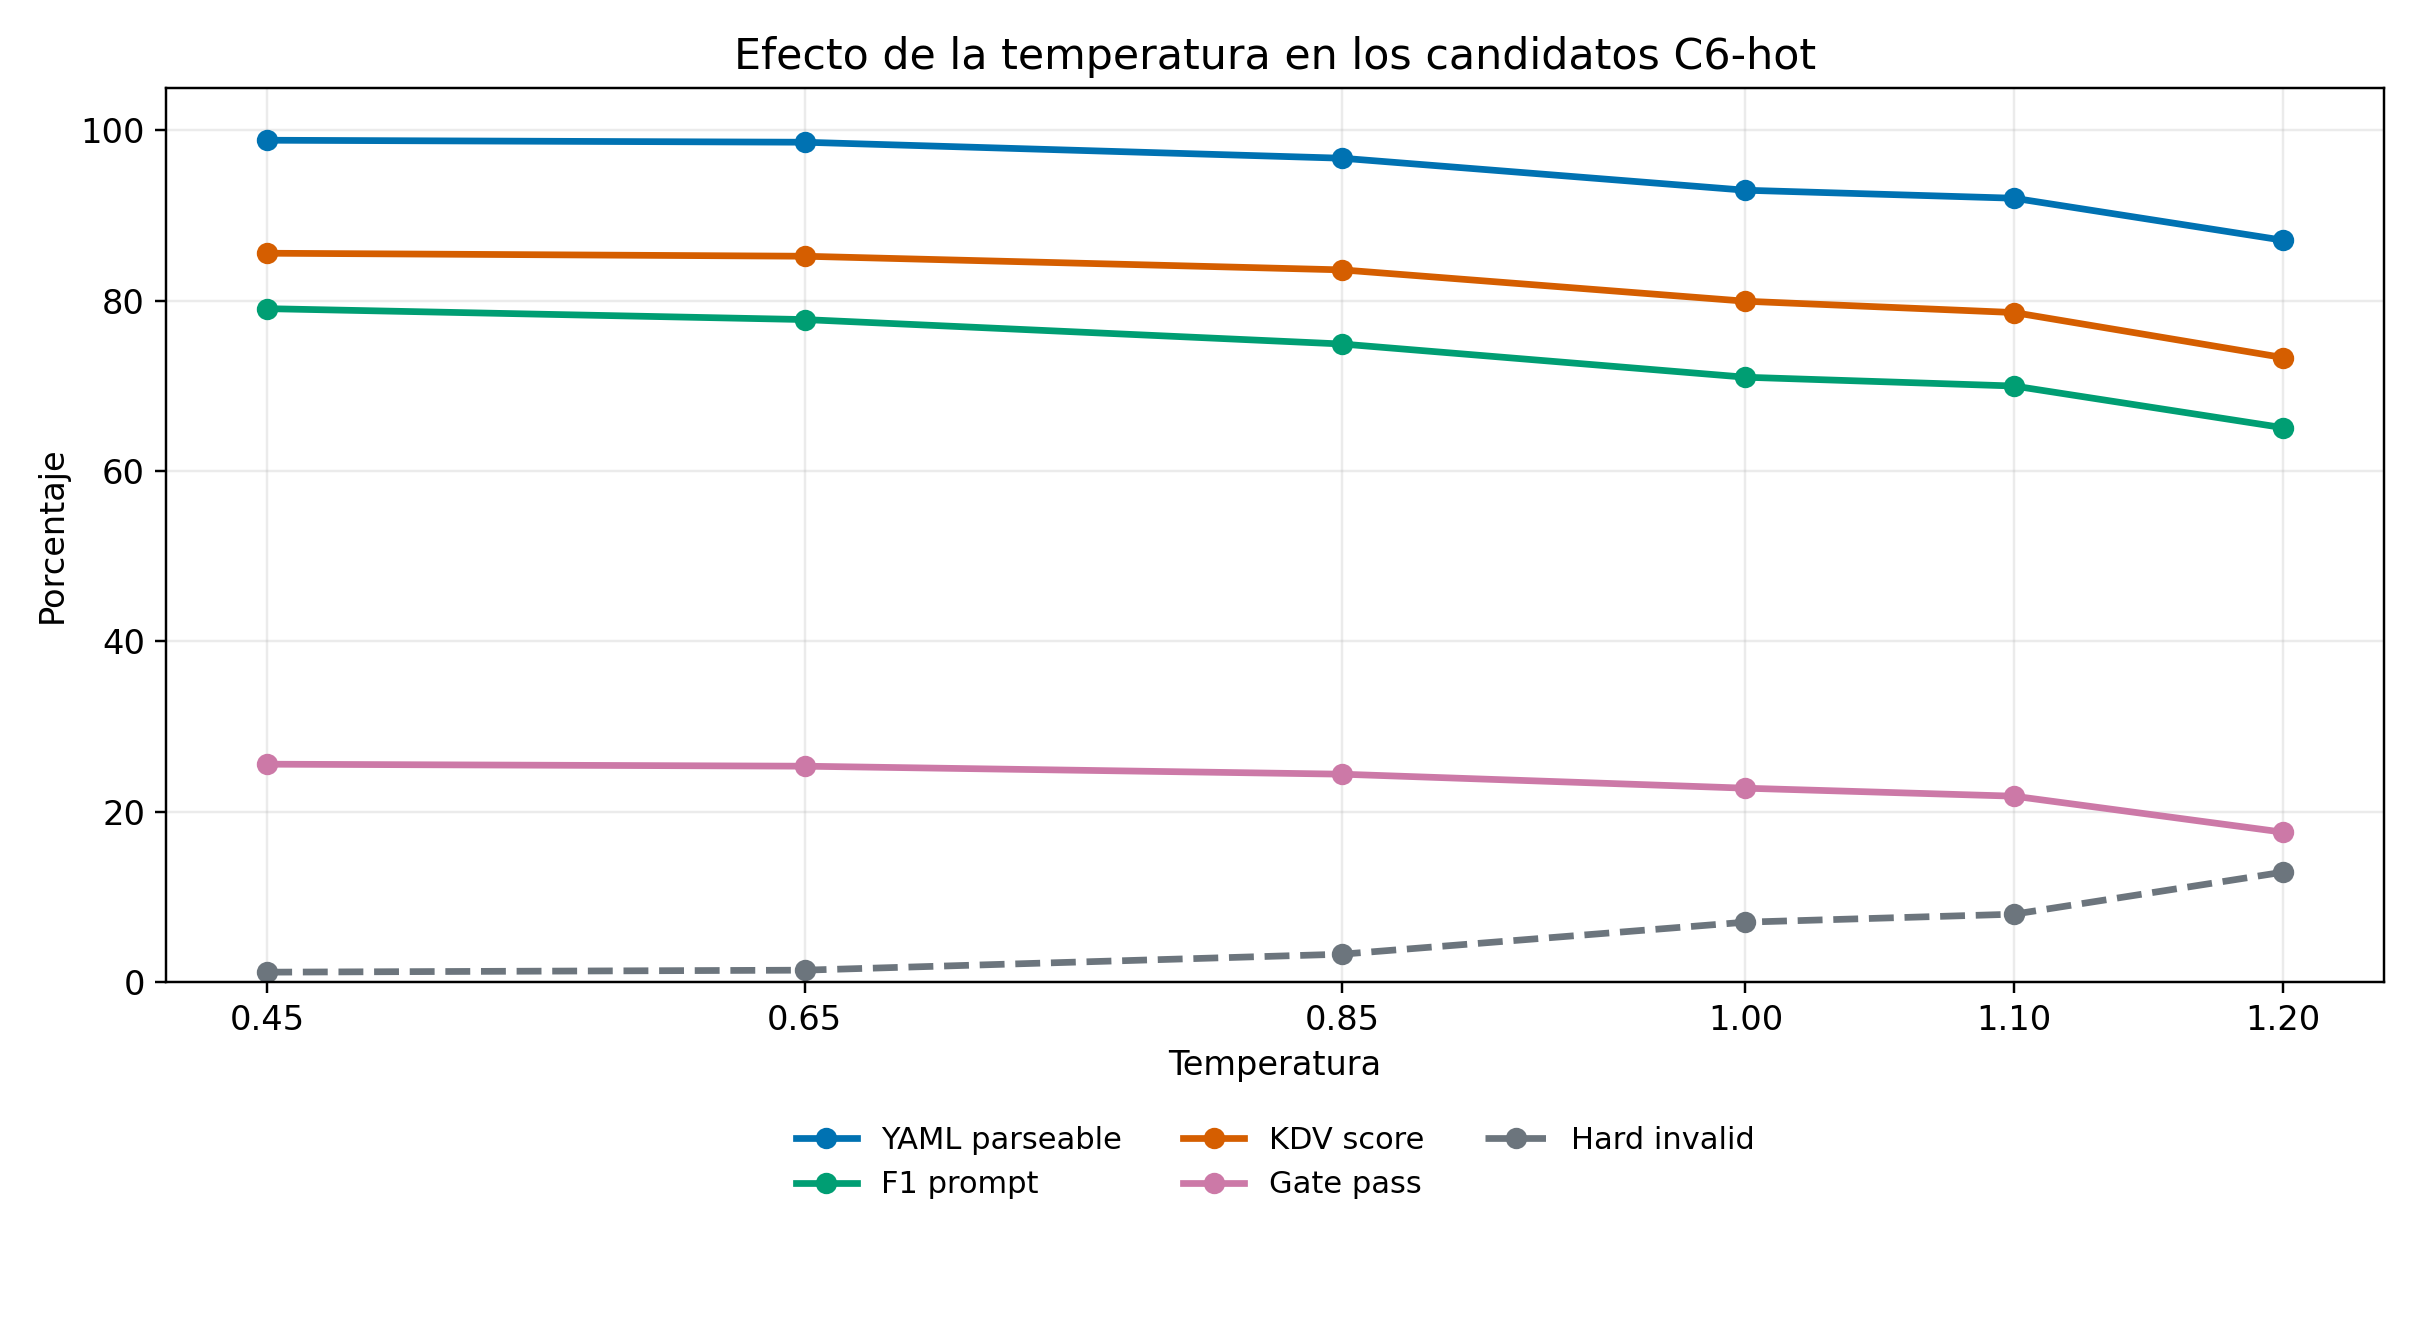
\includegraphics[width=0.92\textwidth]{figures/chapter7/fig7_2_metrics_by_temperature.png}
\caption{Efecto de la temperatura en los candidatos generados con la configuración \texttt{C6 hot}.
         Las temperaturas bajas conservan mejor la calidad media; las temperaturas altas incrementan
         el riesgo de candidatos inválidos y reducen la adecuación al prompt.}
\label{fig:ch7_metrics_by_temperature}
\end{figure}

Esta interpretación se ve con más claridad al observar qué temperatura produce el mejor y el peor
candidato dentro de cada prompt. En la Figura~\ref{fig:ch7_best_worst_temperature}, la temperatura
\(0{,}45\) genera aproximadamente la mitad de los mejores candidatos, mientras que \(1{,}2\) aparece
como peor candidata en casi la mitad de los prompts. La configuración final no busca que todas las
temperaturas sean igual de buenas, sino que el conjunto de seis candidatos contenga una mezcla
razonable de respuestas fuertes, respuestas aceptables y errores útiles para construir contrastes.

\begin{figure}[htbp]
\centering
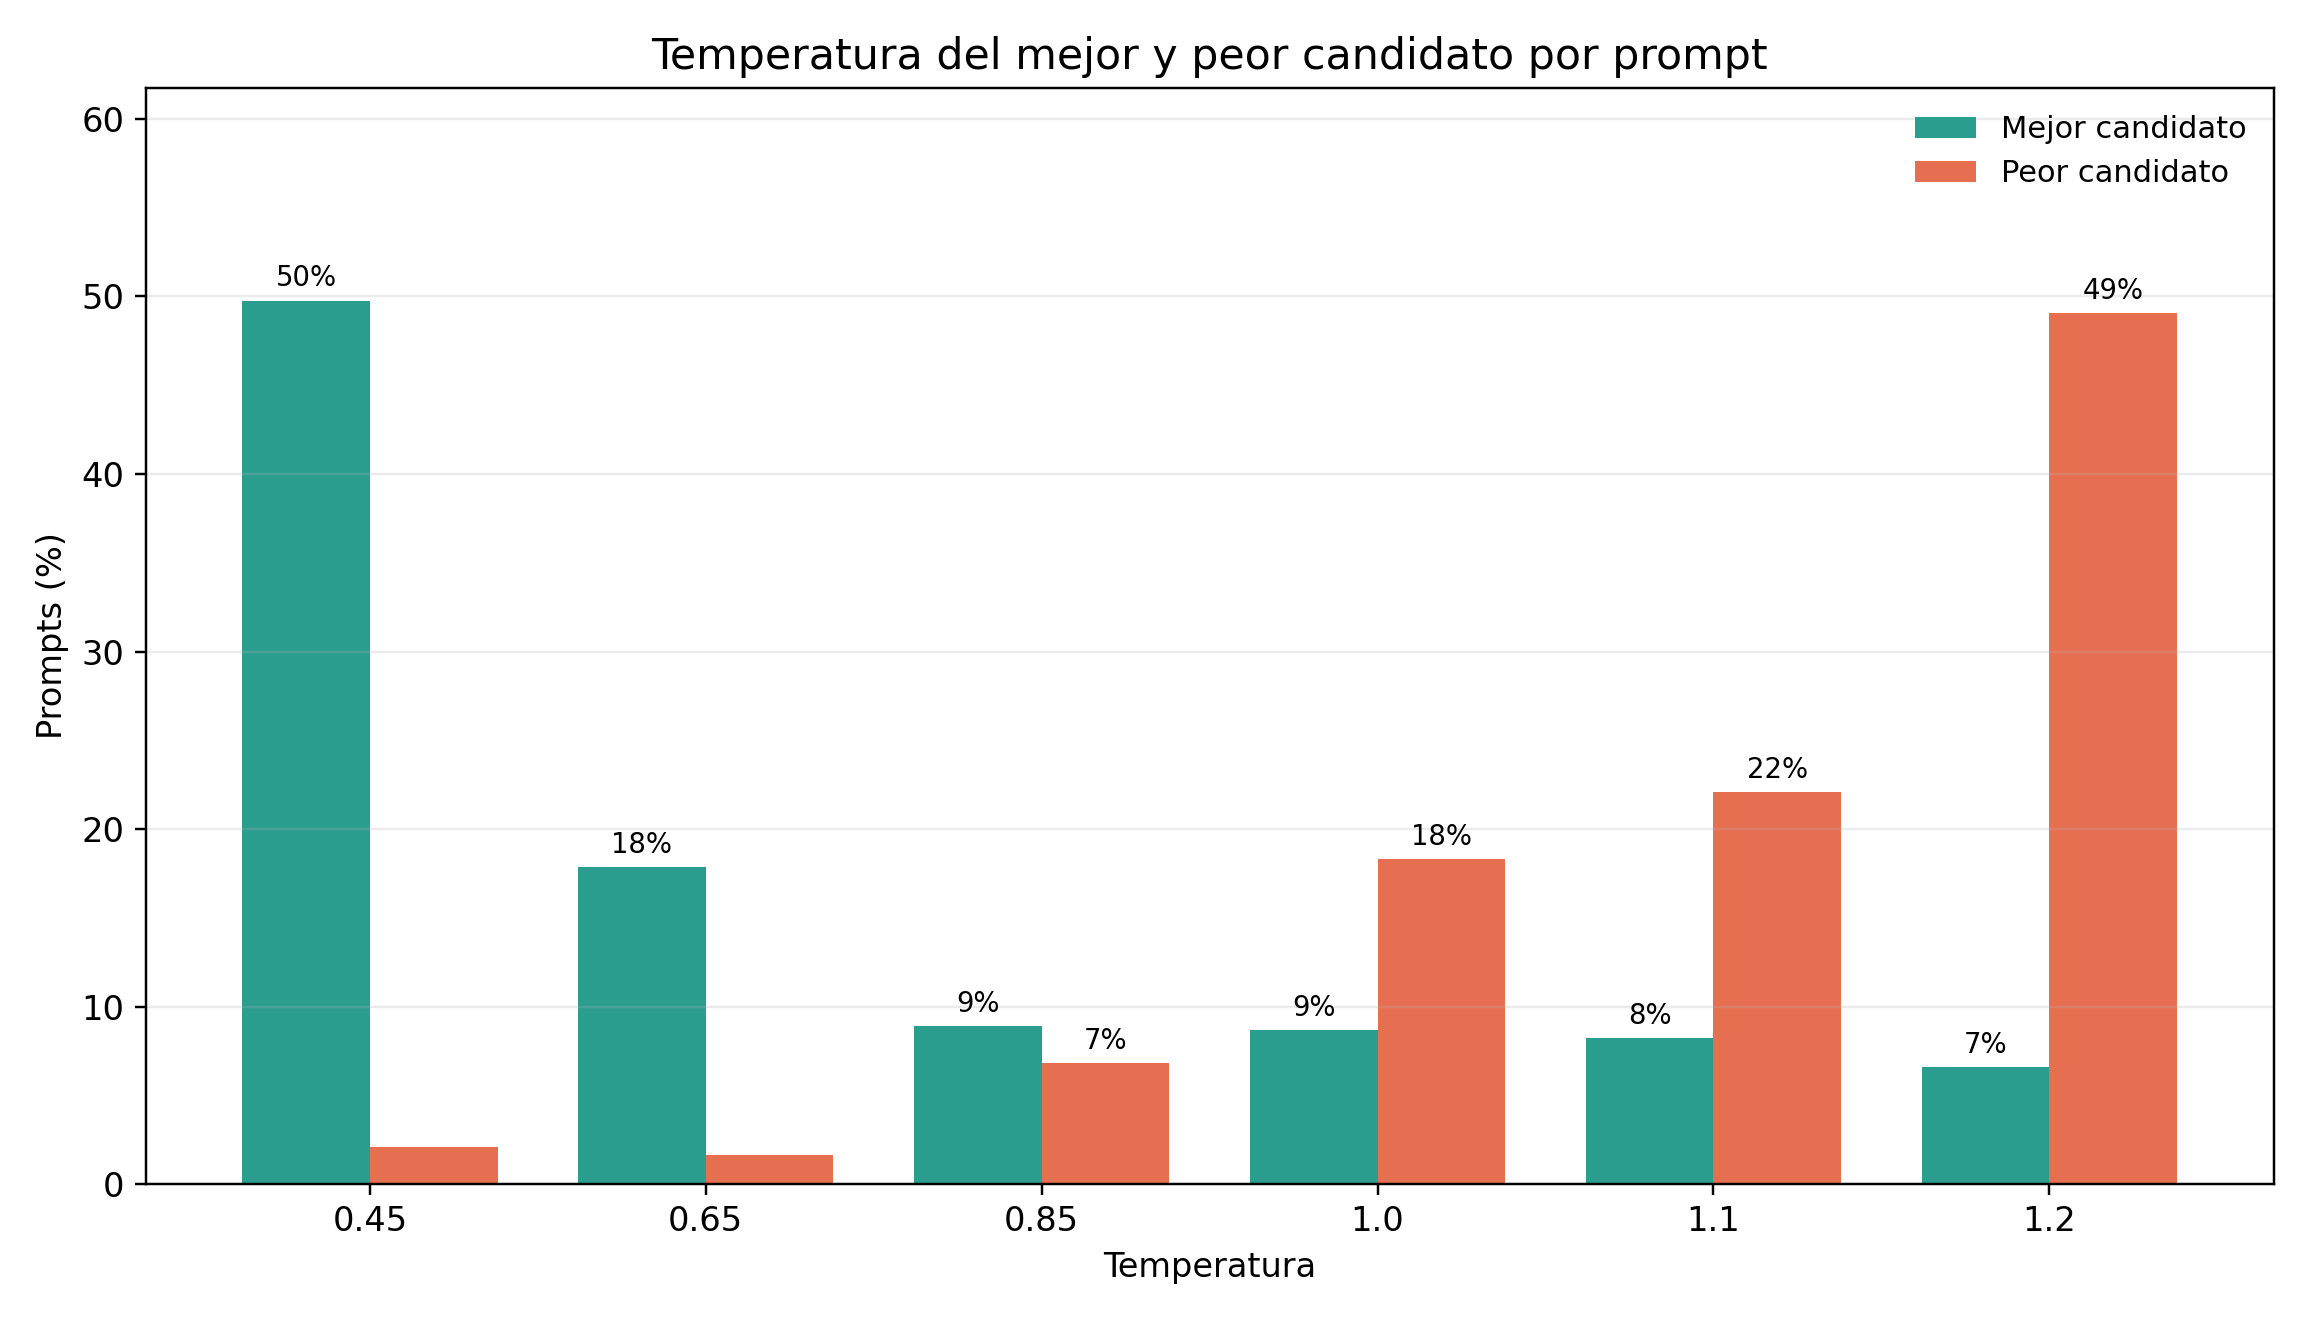
\includegraphics[width=0.86\textwidth]{figures/chapter7/fig7_3_best_worst_temperature.png}
\caption{Temperatura que produce el mejor y el peor candidato por prompt en la generación principal
         \texttt{C6 hot}. La distribución muestra que las temperaturas bajas dominan entre los mejores
         candidatos, mientras que las más altas aportan una parte importante de los peores casos.}
\label{fig:ch7_best_worst_temperature}
\end{figure}

Antes de calcular esos contrastes, cada candidata recibe un score preferencial auxiliar. Para una salida candidata \(y\)
generada ante un prompt \(x\), el score usado en esta fase se define como:

\[
\begin{aligned}
s(y \mid x) ={}&
1{,}00 \cdot \mathrm{PRF1}
+ 0{,}75 \cdot \mathrm{KDV}
+ 0{,}50 \cdot \mathrm{RFC} \\
&+ 0{,}25 \cdot \mathrm{LevelAcc}
+ 0{,}25 \cdot \mathrm{Gate}
- \mathrm{penalizaciones}.
\end{aligned}
\]

En esta expresión, \(\mathrm{PRF1}\) mide la adecuación al prompt, \(\mathrm{KDV}\) resume la
validez de dominio Kubernetes, \(\mathrm{RFC}\) mide la completitud de campos obligatorios,
\(\mathrm{LevelAcc}\) recoge la coincidencia exacta del nivel jerárquico y \(\mathrm{Gate}\)
indica si la candidata supera la compuerta completa de dominio. Las penalizaciones recogen casos
simples pero relevantes, como recursos inventados o diferencias severas en el número de líneas. La
ponderación da prioridad a la adecuación al prompt y después a la validez de dominio, manteniendo la
estructura como señal de retención.

El último criterio fue comprobar si esa diversidad se traducía realmente en pares aprovechables para
DPO. Para cada prompt se calculó la diferencia entre el mejor y el peor score preferencial disponible.
La Figura~\ref{fig:ch7_pair_margin_distribution} muestra que 282 de las 426 unidades de prompt
alcanzan un margen de al menos \(0{,}25\), que es el umbral principal utilizado para conservar pares
con una diferencia suficientemente clara. Otros 21 prompts quedan en el intervalo exploratorio entre
\(0{,}15\) y \(0{,}25\), mientras que 123 no producen contraste suficiente.

\begin{figure}[htbp]
\centering
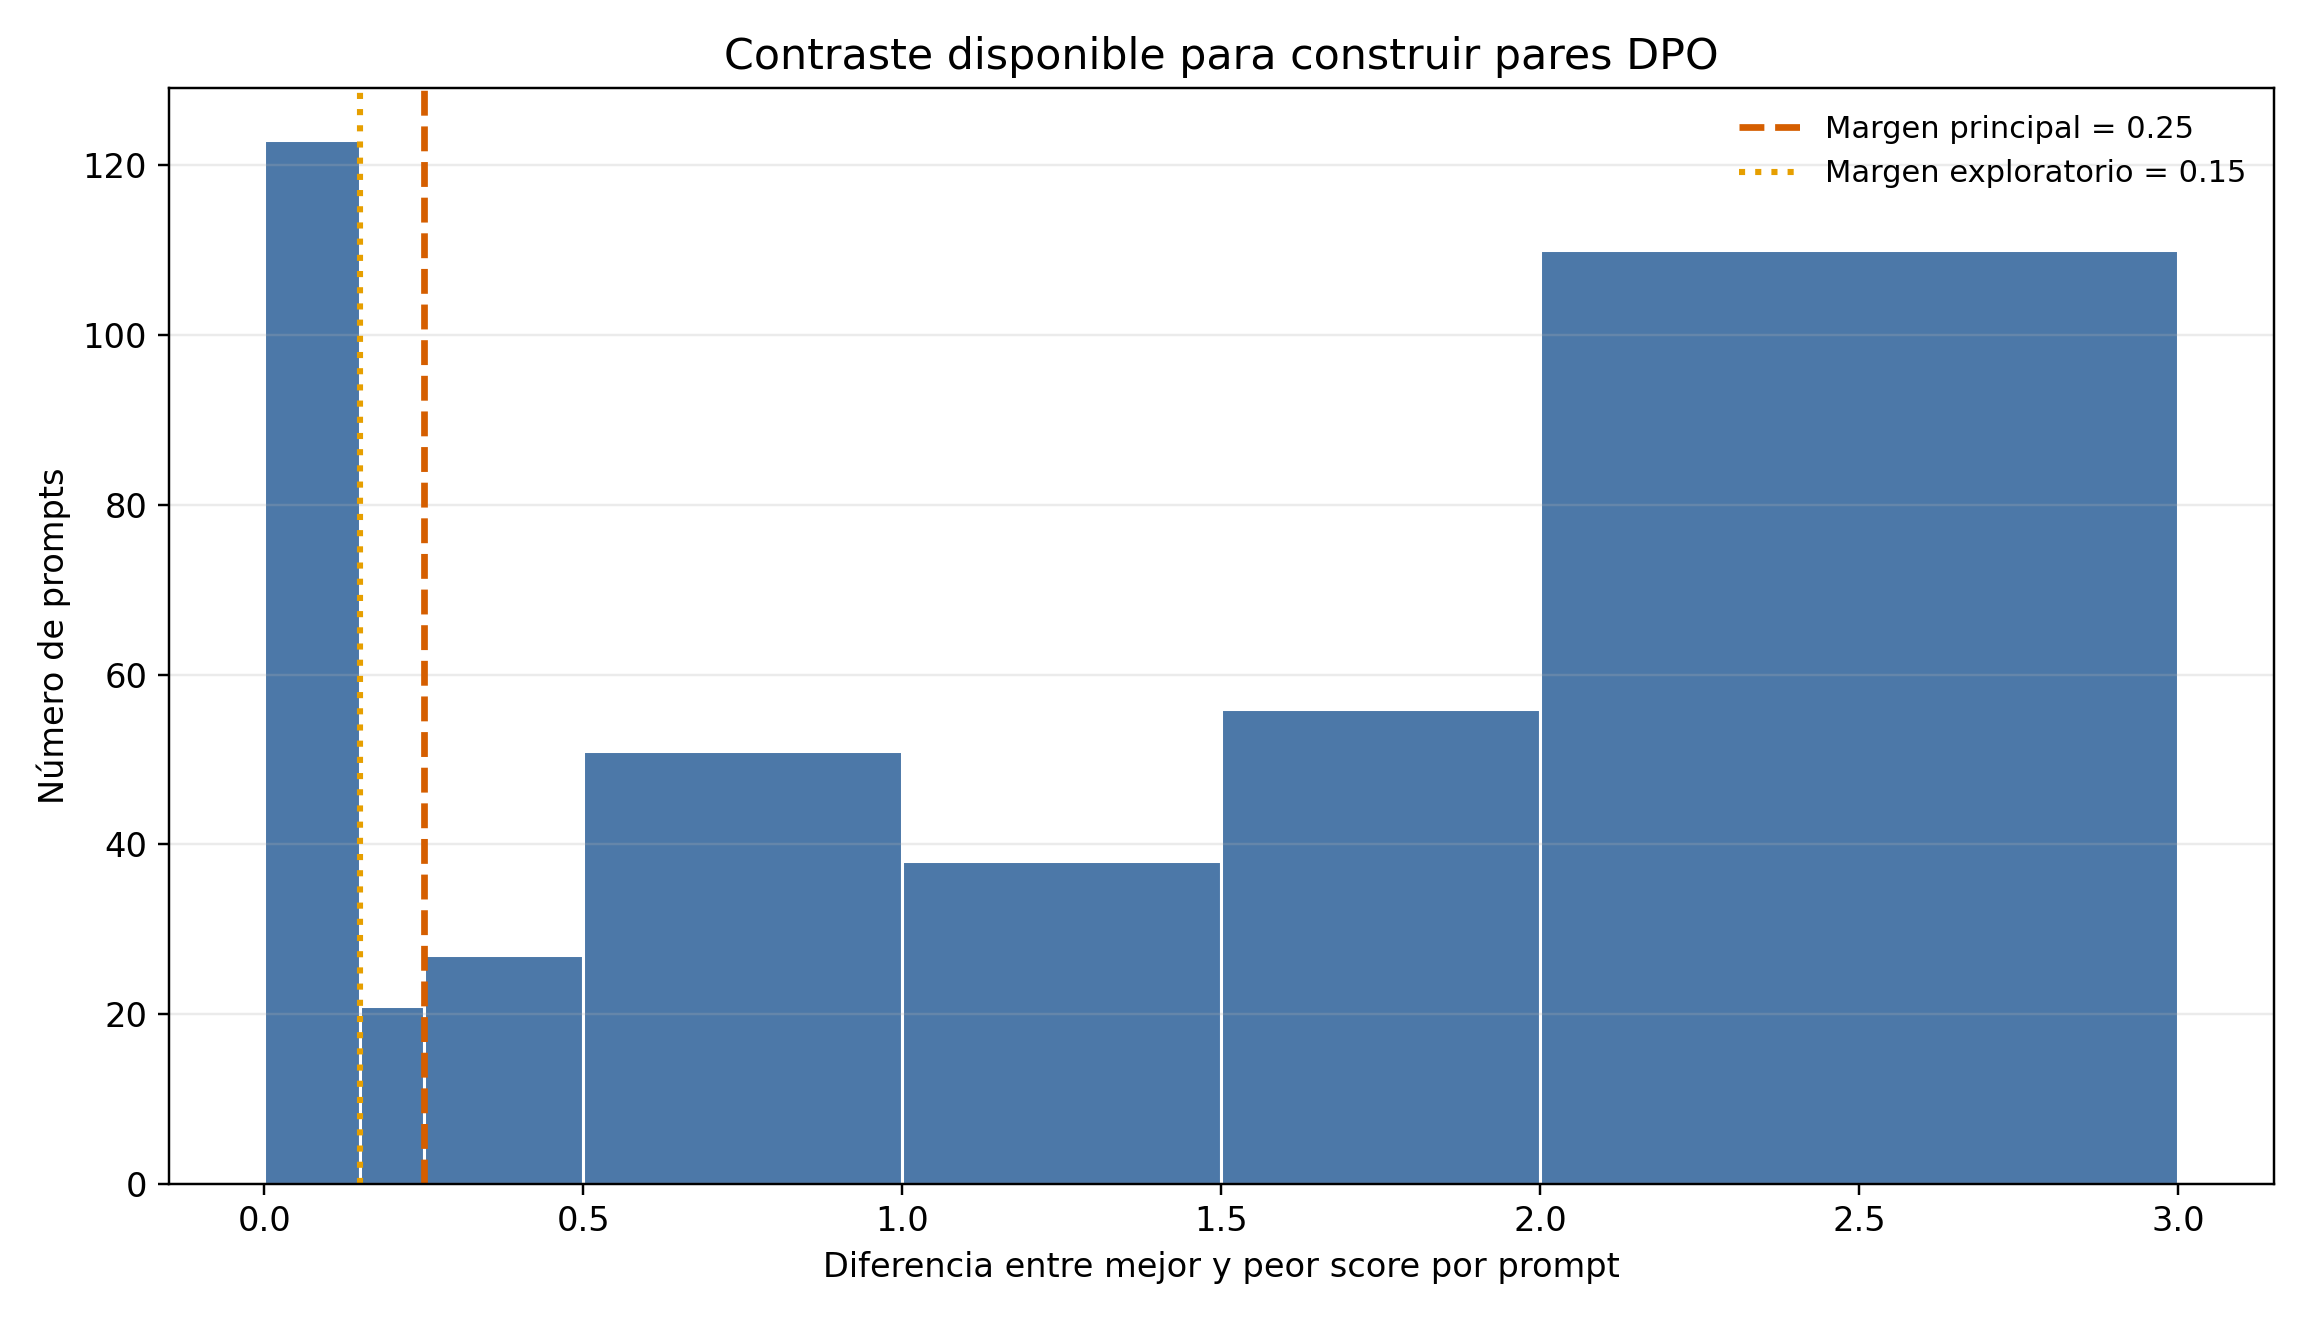
\includegraphics[width=0.88\textwidth]{figures/chapter7/fig7_4_pair_margin_distribution.png}
\caption{Distribución del margen entre el mejor y el peor candidato por prompt. El umbral principal
         de \(0{,}25\) prioriza pares con una diferencia clara, reduciendo el riesgo de entrenar DPO
         con preferencias ambiguas.}
\label{fig:ch7_pair_margin_distribution}
\end{figure}

Con estos resultados se adoptó la estrategia \texttt{C6 hot} para la generación principal de
candidatos. La decisión no se basa en que sea la configuración con mejor calidad media, sino en que
ofrece una combinación más útil para una etapa de preferencias: mantiene una tasa alta de
parseabilidad, reduce duplicados respecto al rango \texttt{wide} y genera suficientes diferencias
entre candidatos como para seleccionar pares \texttt{chosen}/\texttt{rejected}.

%----------------------------------------------------------------------
\section{Primer ajuste DPO sobre el dataset de preferencias V1}
\label{sec:ch7_dpo_v1}
%----------------------------------------------------------------------

A partir de la generación anterior se construyó el primer conjunto de preferencias DPO. El dataset
final contiene 454 tripletas \((x,y^+,y^-)\), distribuidos sobre 230 prompts de entrenamiento. En cada tripleta,
\(y^+\) representa la candidata preferida y \(y^-\) la candidata rechazada. La selección la hize a través
una interfaz desarrollada ad hoc, que permitía visualizar los candidatos de cada prompt con sus métricas y
su valor de puntuación, de modo que podía elegir el par más informativo para cada unidad de prompt en base a
mi criterio y al score preferencial definido en la sección anterior.

Formalmente, DPO ajusta una política \(\pi_\theta\) frente a una política de referencia
\(\pi_{\mathrm{ref}}\). Para cada tripleta de preferencia, la pérdida usada por DPO puede escribirse
como:

\[
\mathcal{L}_{\mathrm{DPO}}(\theta)=
-\mathbb{E}_{(x,y^+,y^-)\sim \mathcal{D}}
\left[
\log \sigma
\left(
\beta
\left[
\log \frac{\pi_\theta(y^+ \mid x)}{\pi_{\mathrm{ref}}(y^+ \mid x)}
-
\log \frac{\pi_\theta(y^- \mid x)}{\pi_{\mathrm{ref}}(y^- \mid x)}
\right]
\right)
\right].
\]

La expresión anterior es útil porque hace visible el papel de \(\beta\). Un valor menor suaviza la
actualización y restringe más el desplazamiento respecto a la referencia; un valor mayor permite que
la diferencia entre la respuesta preferida y la rechazada pese más en la actualización. En este
trabajo se probaron dos valores, \(\beta=0{,}10\) y \(\beta=0{,}30\), manteniendo como referencia el
modelo de partida \texttt{serialized\_sft}.

TODO AQUÍ

\begin{table}[htbp]
\centering
\small
\begin{tabularx}{\textwidth}{Xrrr}
\toprule
\textbf{Métrica de validación} &
\textbf{\texttt{serialized\_sft}} &
\textbf{DPO \(\beta=0{,}10\)} &
\textbf{DPO \(\beta=0{,}30\)} \\
\midrule
YAML parseable & 98,57\,\% & 97,14\,\% & pendiente \\
Bloques parseables & 98,57\,\% & 97,14\,\% & pendiente \\
Manifiesto reconstruido exacto & 11,43\,\% & 14,29\,\% & pendiente \\
Coincidencia en número de documentos & 92,86\,\% & 94,29\,\% & pendiente \\
F1 medio de líneas & 0,8206 & 0,8092 & pendiente \\
Exactitud media de \texttt{level} & 0,7578 & 0,7422 & pendiente \\
F1 medio de requisitos del prompt & 0,8531 & 0,8368 & pendiente \\
F1 medio de claves semánticas & 0,9552 & 0,9406 & pendiente \\
Score KDV medio & 0,8310 & 0,8286 & pendiente \\
\textit{Domain gate} completo & 14,29\,\% & 12,86\,\% & pendiente \\
Nivel KDV medio & 3,9000 & 3,9429 & pendiente \\
\bottomrule
\end{tabularx}
\caption{Comparación de validación entre el modelo de partida y DPO con \(\beta=0{,}10\). La columna
         de \(\beta=0{,}30\) se mantiene como marcador de resultados pendientes, porque la evaluación
         completa sobre los 70 ejemplos de validación no estaba disponible en el momento de redactar
         esta sección.}
\label{tab:ch7_dpo_v1_validation}
\end{table}

TODO AQUÍ

%----------------------------------------------------------------------
\section{Generación iterativa del dataset DPO v2}
\label{sec:ch7_dpo_v2_generation}
%----------------------------------------------------------------------

\subsection{Planteamiento del enfoque iterativo}

El paso a DPO v2 se plantea como el inicio de un procedimiento iterativo de alineación ligera. La
idea es aprovechar una propiedad práctica del aprendizaje por refuerzo en metodologías on-line: una vez obtenida una política ajustada,
esa política puede usarse para generar nuevos candidatos y revelar una distribución de errores
distinta a la observada antes del ajuste. En términos de la literatura de optimización por
preferencias, se mantiene la simplicidad offline de DPO \citep{rafailov2023dpo}, pero se actualiza el
origen de los candidatos entre iteraciones. Esto permite atacar uno de los puntos débiles del método de DPO: la política de referencia permanece 
fija mientras que la distribución de los candidatos evoluciona.

El esquema iterativo puede describirse como una sucesión de políticas
\(\pi_{\theta_0}, \pi_{\theta_1}, \ldots\). La política inicial
\(\pi_{\theta_0}\) corresponde a \texttt{serialized\_sft}. Tras entrenar DPO v1 se obtiene
\(\pi_{\theta_1}\). En la siguiente iteración, los candidatos ya no se muestrean desde
\(\pi_{\theta_0}\), sino desde la política ajustada:

\[
y_{i,j}^{(t)} \sim \pi_{\theta_{t-1}}(\cdot \mid x_i),
\qquad j=1,\ldots,k.
\]

Sobre esos candidatos se construye un nuevo conjunto de preferencias:

\[
\mathcal{D}_{\mathrm{pref}}^{(t)} =
\left\{
\left(x_i,y_i^+,y_i^-\right)
:
S_t(y_i^+ \mid x_i)-S_t(y_i^- \mid x_i) \geq \delta_t
\right\}.
\]

Aquí \(S_t\) representa el score preferencial de la iteración \(t\), \(\delta_t\) es el margen mínimo
exigido entre la salida preferida y la rechazada. Estas restricciones son importantes porque impiden que un par se
conserve solo por mejorar una métrica aislada si al mismo tiempo empeora demasiado la fidelidad al
prompt o la estructura de bloques. Finalmente, la siguiente política se entrena con una referencia
actualizada:

\[
\pi_{\mathrm{ref}}^{(t)}=\pi_{\theta_{t-1}},
\qquad
\theta_t =
\arg\min_{\theta}
\mathcal{L}_{\mathrm{DPO}}^{(t)}
\left(
\theta;
\mathcal{D}_{\mathrm{pref}}^{(t)},
\pi_{\mathrm{ref}}^{(t)}
\right).
\]

La Figura~\ref{fig:ch7_dpo_iterative_cycle} resume esta idea en forma de esquema. El punto central es que el ciclo no
promete una mejora automática en cada vuelta. Lo que permite es hacer que el siguiente dataset de
preferencias esté condicionado por los errores de la política que realmente se quiere seguir
ajustando. En concreto para mi tarea, esto puede resultar más útil y producir mejores resultados que repetir
indefinidamente pares producidos por el modelo SFT inicial, cuyos \textit{gaps} pueden haber sido ya corregidos.

\begin{figure}[htbp]
\centering
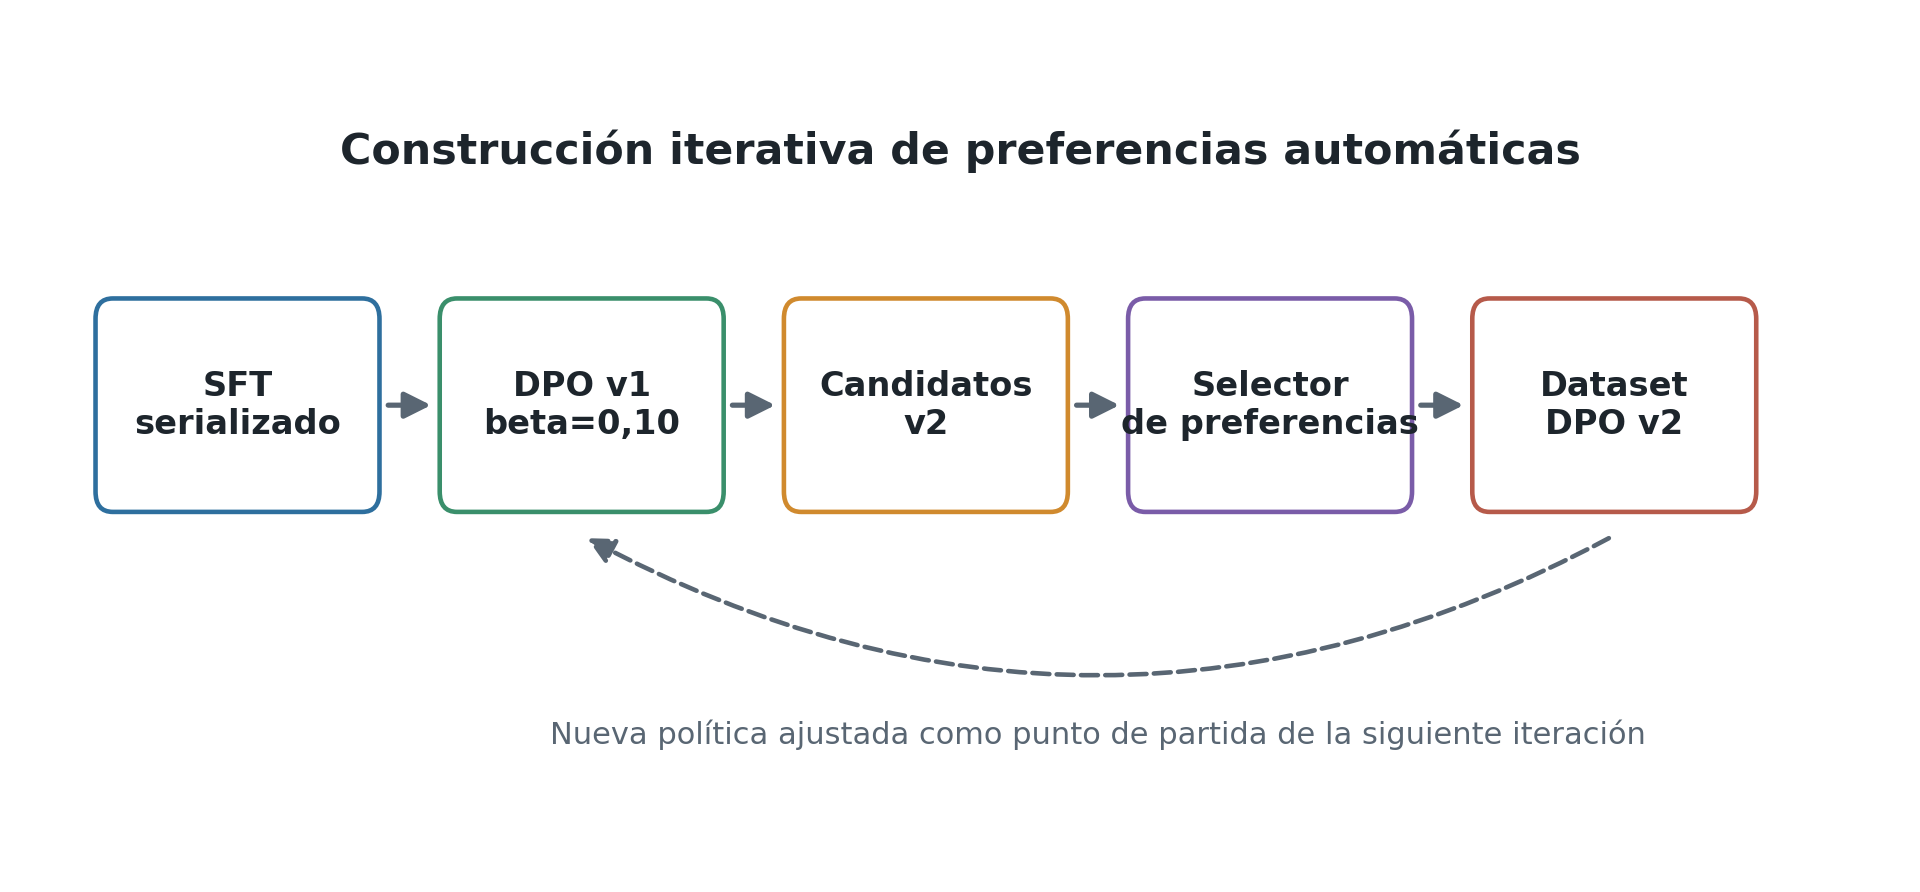
\includegraphics[width=0.95\textwidth]{figures/chapter7/fig7_5_dpo_iterative_cycle.png}
\caption{Esquema iterativo seguido para pasar de DPO v1 a la generación del dataset DPO v2. La nueva
         política se usa para muestrear candidatos y la política anterior actúa como referencia de la
         siguiente actualización.}
\label{fig:ch7_dpo_iterative_cycle}
\end{figure}

\subsection{Construcción del dataset DPO V2}

En la práctica, DPO v2 se generó a partir del modelo final de la ejecución con \(\beta=0{,}10\). 
Se mantuvieron los 426 prompts de entrenamiento como universo de generación y se
produjeron seis candidatos por prompt, con el mismo espíritu de diversidad controlada de la fase
anterior. La diferencia está en la intuición que usé para el etiquetado. Cuando estudié las métricas en el dataset 
v1 vi que predominaban pares de margen amplio y negativos
intermedios. Sin embargo, en el dataset v2 busqué que los contrastes fueran más diagnósticos: cruces de compuerta
Kubernetes, práctica de nivel KDV 5, invariantes de dominio, fidelidad al prompt y fidelidad
estructural.

\begin{table}[htbp]
\centering
\small
\begin{tabularx}{\textwidth}{Xrr}
\toprule
\textbf{Elemento} & \textbf{DPO v1} & \textbf{DPO v2} \\
\midrule
Política usada para generar candidatos & \texttt{serialized\_sft} & DPO v1 \(\beta=0{,}10\) \\
Prompts de entrenamiento considerados & 426 & 426 \\
Candidatos evaluados & 2556 & 2556 \\
Pares finales & 454 & 229 \\
Prompts con al menos un par & 230 & 193 \\
Margen preferencial medio & 0,9310 & 1,0078 \\
Diferencia media de F1 de prompt & 0,1454 & 0,1732 \\
Diferencia media de F1 de líneas & 0,1780 & 0,2665 \\
Diferencia media de exactitud de \texttt{level} & 0,2455 & 0,3124 \\
Pares de cruce de compuerta & 40 & 62 \\
Cruces con deriva de prompt & 20 & 1 \\
\bottomrule
\end{tabularx}
\caption{Comparación entre los datasets de preferencias DPO v1 y DPO v2. DPO v2 conserva menos pares,
         pero los pares retenidos tienen mayor margen medio y están más orientados a fallos
         estructurales y de dominio.}
\label{tab:ch7_dpo_v1_v2_dataset_summary}
\end{table}

No debemos interpretar la reducción de 454 a 229 pares como una pérdida de datos, sino como una selección más
cuidadosa. Se supone que el modelo DPO v1 ya habrá corregido parte de los errores más evidentes, por lo que el
siguiente paso es centrarse en los contrastes más específicos de dominio y estructura. La
Tabla~\ref{tab:ch7_dpo_v2_guardrails} muestra las principales restricciones en las que me apoyé para aceptar un
par. Todas ellas comparan la salida preferida con la rechazada y funcionan como barreras contra
mejoras aparentes: por ejemplo, nunca aceptaré una candidata como \textit{chosen} si gana en dominio
pero pierde demasiada fidelidad al prompt o destruye la estructura de bloques.

\begin{table}[htbp]
\centering
\small
\begin{tabularx}{\textwidth}{lX}
\toprule
\textbf{Restricción} & \textbf{Criterio de aceptación} \\
\midrule
Margen mínimo & \(S(y^+ \mid x)-S(y^- \mid x) \geq 0{,}25\) \\
Fidelidad al prompt & \(\mathrm{PRF1}(y^+) \geq \mathrm{PRF1}(y^-) - 0{,}05\) \\
Texto de líneas & \(\mathrm{LineF1}(y^+) \geq \mathrm{LineF1}(y^-) - 0{,}10\) \\
Jerarquía \texttt{level} & \(\mathrm{LevelAcc}(y^+) \geq \mathrm{LevelAcc}(y^-) - 0{,}15\) \\
Campos obligatorios & \(\mathrm{ReqFields}(y^+) \geq \mathrm{ReqFields}(y^-) - 0{,}05\) \\
\bottomrule
\end{tabularx}
\caption{Restricciones principales del selector DPO v2. El objetivo no es maximizar una sola métrica,
         sino evitar pares donde la preferencia sea contradictoria con el contrato estructural de la
         tarea.}
\label{tab:ch7_dpo_v2_guardrails}
\end{table}

La composición de tipos de pares cambia de forma clara entre ambas iteraciones. Como se observa en la
Figura~\ref{fig:ch7_dpo_v1_v2_pair_types}, el dataset DPO v1 estaba dominado por pares de margen amplio y
negativos intermedios. El dataset DPO v2, en cambio, reparte la señal entre invariantes de dominio, cruces de
compuerta, fidelidad al prompt y fidelidad estructural. Esta era la idea que queríamos seguir: 
si \(\beta=0{,}10\) ya corrige parte de los contrastes más evidentes, la siguiente
iteración debe concentrarse en errores más cercanos a la frontera de validez.

\begin{figure}[htbp]
\centering
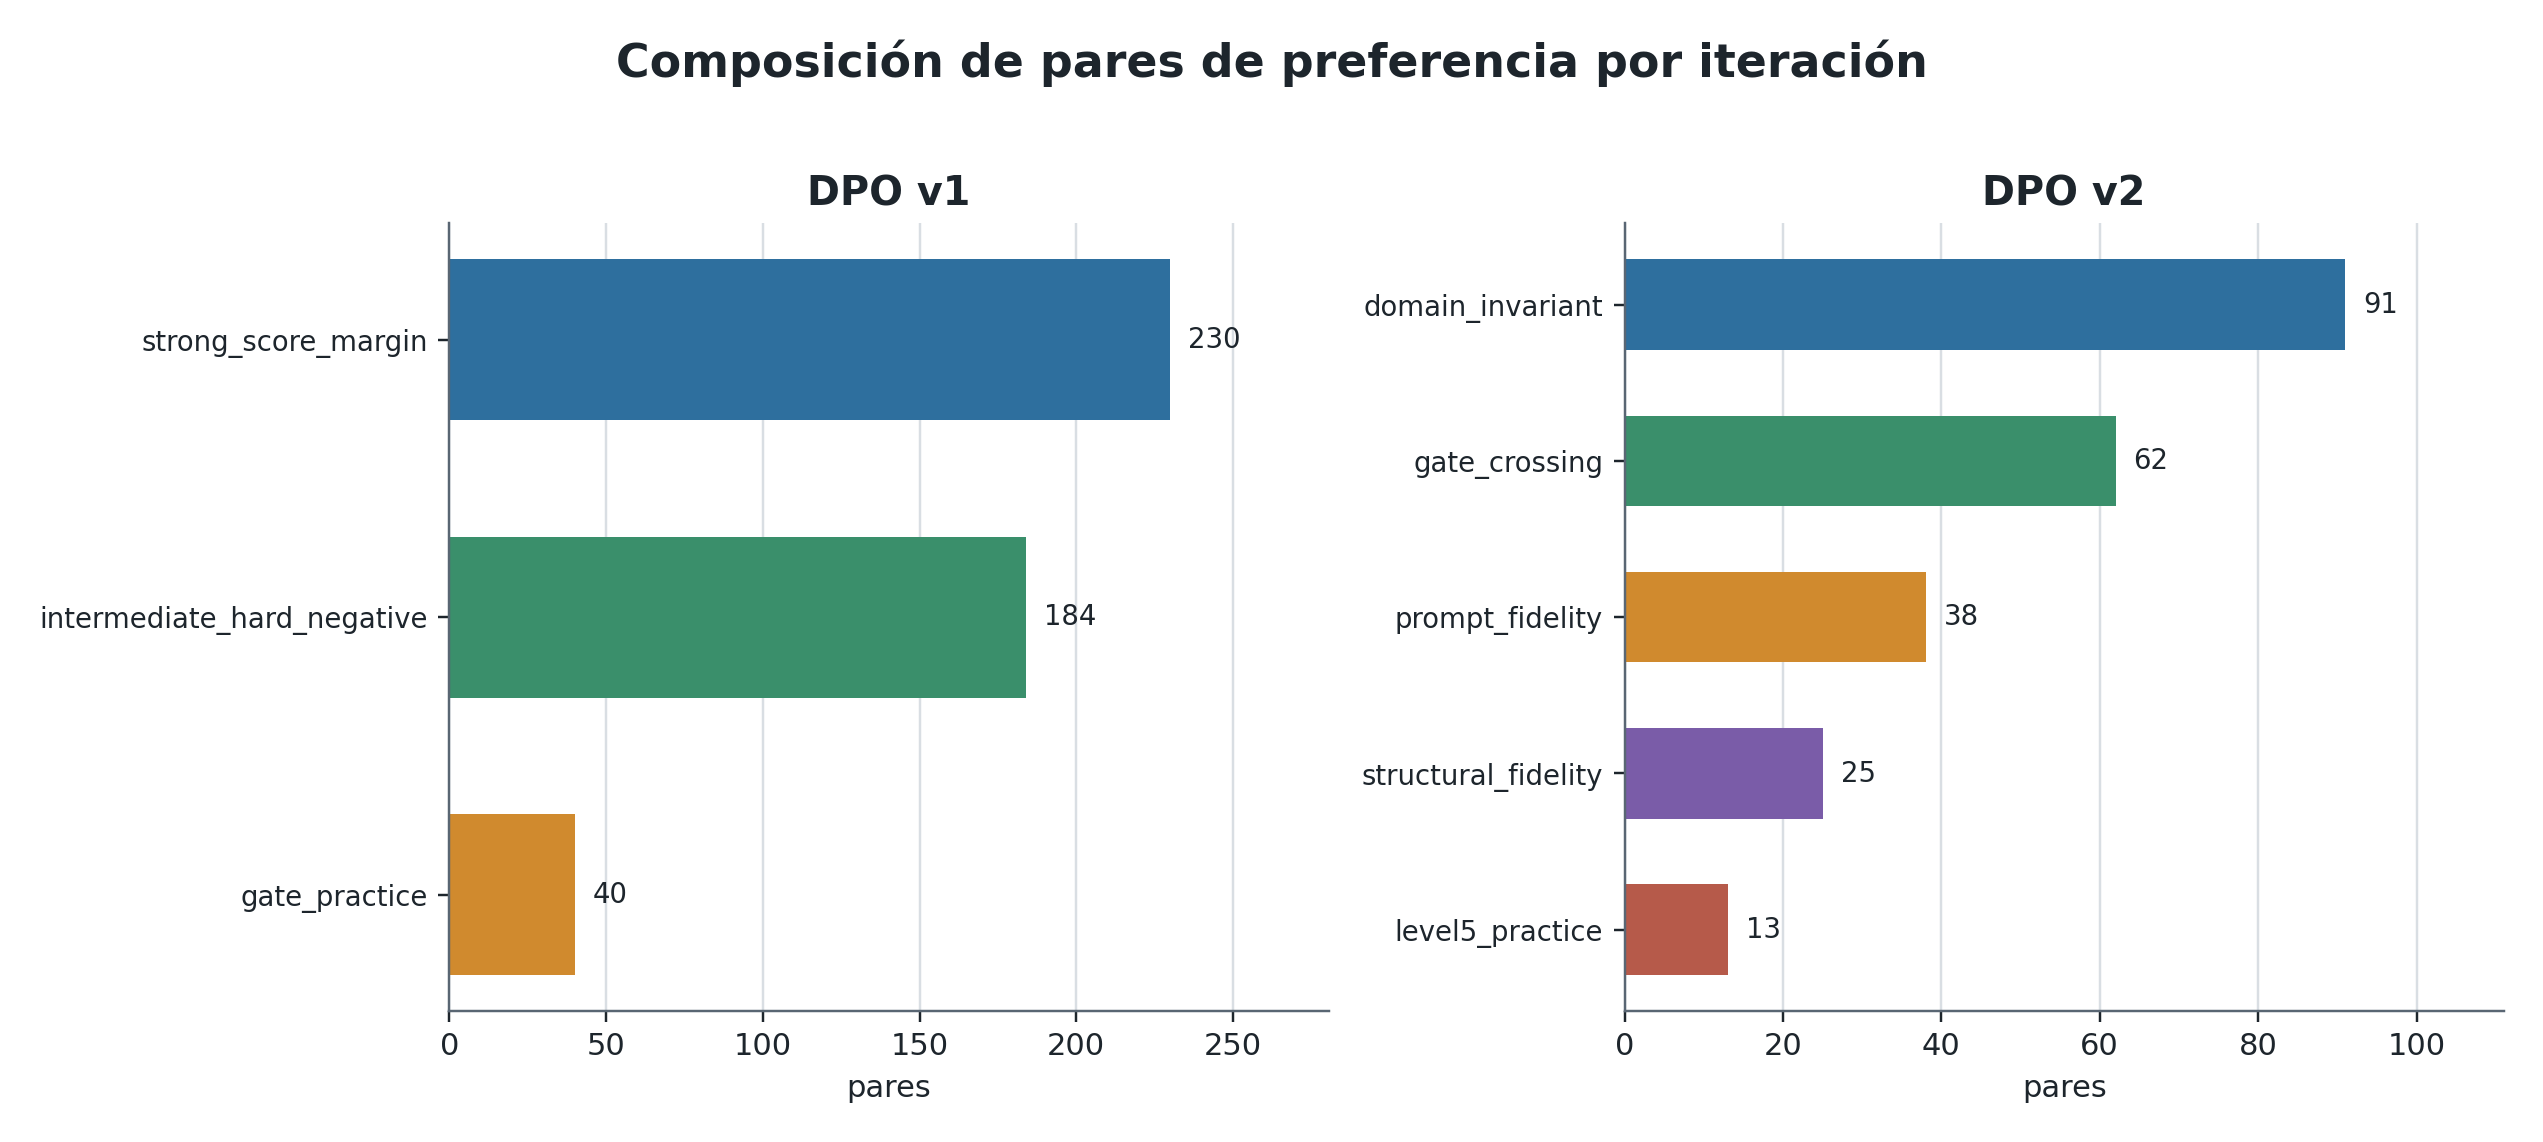
\includegraphics[width=\textwidth]{figures/chapter7/fig7_6_dpo_v1_v2_pair_types.png}
\caption{Composición de tipos de pares en DPO v1 y DPO v2. La segunda iteración reduce el número
         total de pares, pero desplaza el foco hacia contrastes más específicos de dominio y
         estructura.}
\label{fig:ch7_dpo_v1_v2_pair_types}
\end{figure}

El mismo cambio se aprecia al mirar la distribución de niveles KDV. En el dataset DPO v2, las respuestas
preferidas se concentran en los niveles 4 y 5, mientras que las rechazadas se acumulan sobre todo en
el nivel 1. Esta es una condición necesaria para que la pérdida DPO pueda
aprender una dirección útil: si \(y^+\) e \(y^-\) son demasiado parecidos o fallan por motivos
opuestos, el gradiente resultante es menos interpretable.

\begin{figure}[htbp]
\centering
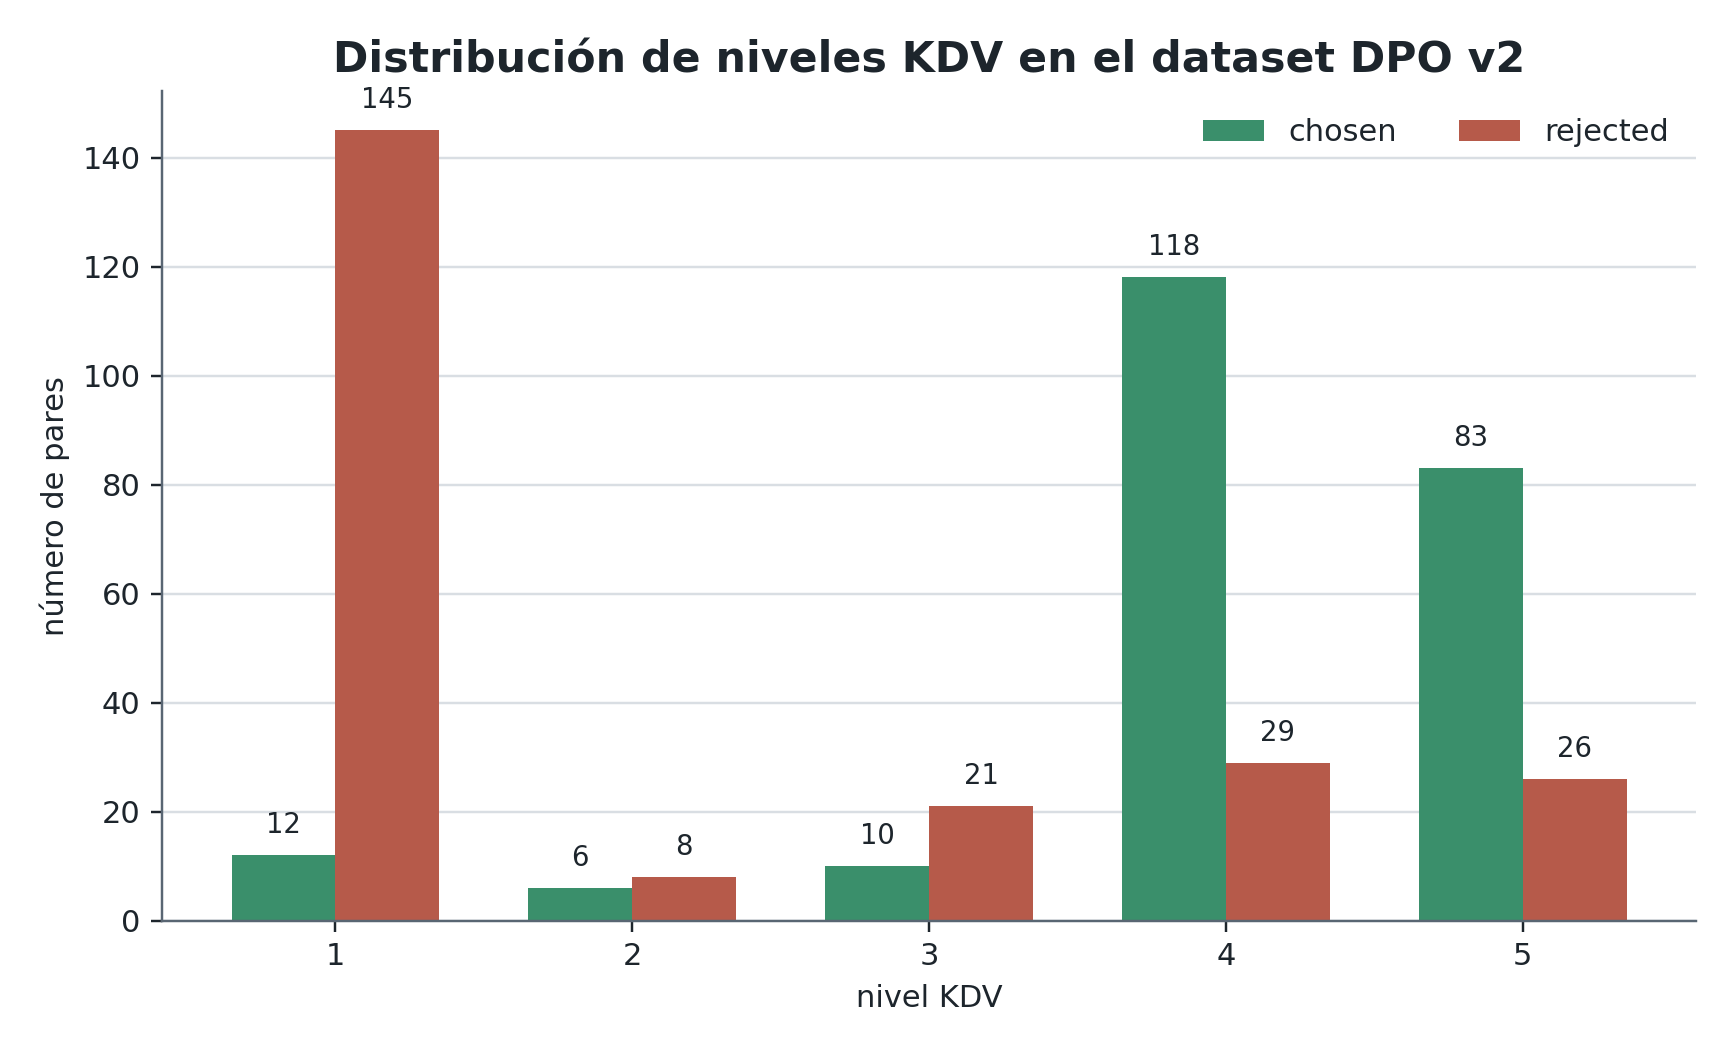
\includegraphics[width=0.86\textwidth]{figures/chapter7/fig7_7_dpo_v2_kdv_levels.png}
\caption{Distribución de niveles KDV entre salidas preferidas y rechazadas en DPO v2. Los
         \textit{chosen} se concentran en niveles altos, mientras que los \textit{rejected} contienen
         una proporción elevada de fallos de dominio severos.}
\label{fig:ch7_dpo_v2_kdv_levels}
\end{figure}

Por último, la separación media entre \textit{chosen} y \textit{rejected} muestra que la segunda
iteración no solo introduce pares de dominio, sino también diferencias estructurales más marcadas. La
Figura~\ref{fig:ch7_dpo_v2_metric_deltas} resume las diferencias medias en algunas de las métricas.
La mejora relativa en exactitud de \texttt{level} y F1 de líneas es
especialmente relevante para este caso, porque conecta la etapa de preferencias con la hipótesis
central de la que partimos: la salida no debe evaluarse como una cadena plana, sino como una representación
que tiene que preservar una jerarquía reconstruible.

\begin{figure}[htbp]
\centering
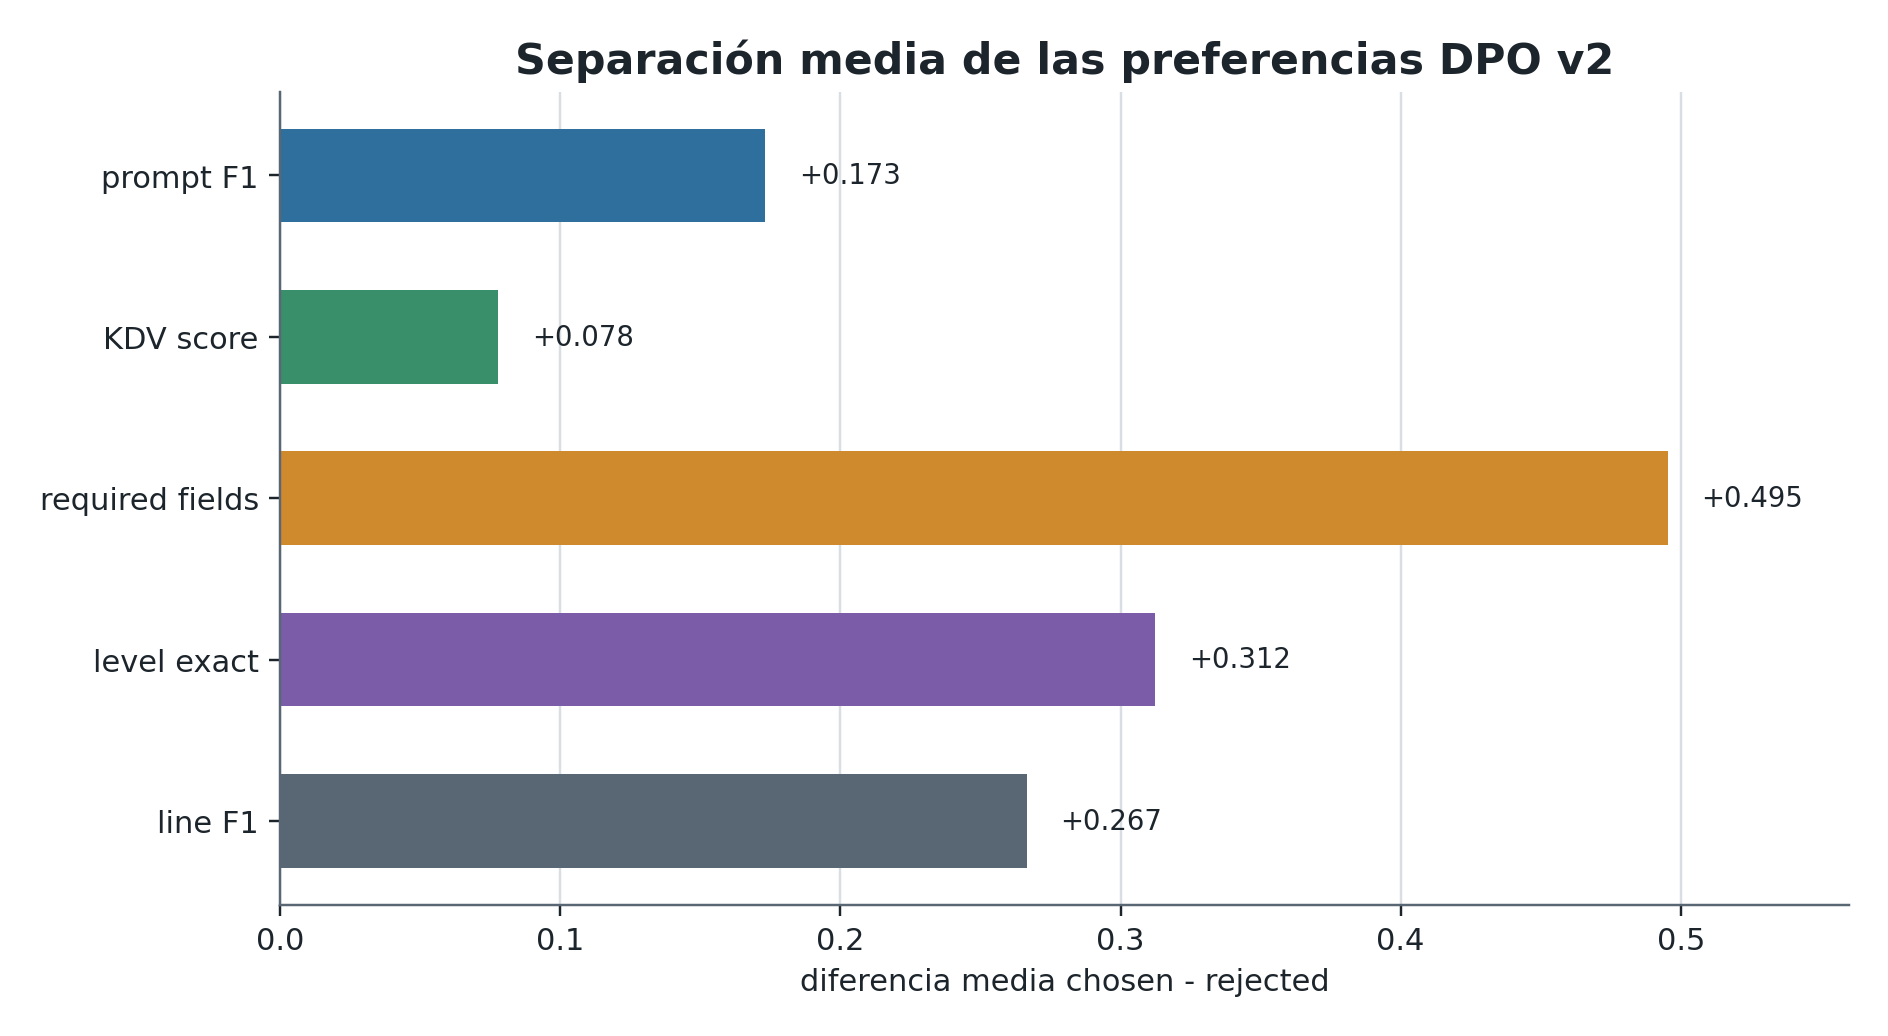
\includegraphics[width=0.86\textwidth]{figures/chapter7/fig7_8_dpo_v2_metric_deltas.png}
\caption{Diferencia media entre salida preferida y salida rechazada en el dataset DPO v2. Las
         diferencias positivas indican que el selector conserva pares donde la preferencia está
         apoyada por varias señales y no por una sola métrica aislada.}
\label{fig:ch7_dpo_v2_metric_deltas}
\end{figure}

\section{Segundo ajuste DPO sobre dataset de preferencias V2}
